	\section{Impact of missing data}
		\subsection{Is less missing data always better?}
	\label{miss_impact}
	\todo{Ajouter une erreur de référence: au meilleur de la prédiction, on est bons?}
%When estimating a model parameter, we generally want as little missing data as possible
%Especially, when the missing data pattern is MCAR and we have lots of complete cases, it is tempting to use just them
%However, it is possible that we really need to have the same MD pattern for train and validation (real-world data), as illustrated by empirical results: with mean imputation, the best predicition is when  there  is the same amount in both sets!
When performing an analysis, it is intuitive that we should limit the amount of missing data as much as possible, since missing data pollutes our estimates.

In particular, if the missing data is MCAR --- and so the complete cases have exactly the same distribution as those with missing data ---, and we have a large enough dataset with many complete cases (as in the Traumabase), it is tempting to use only those complete cases to learn our model. Even in a context where we are training for prediction, and the real-world data will have some missing values we need to handle, it seems that we can use complete cases in the training data to learn both our prediction and imputation parameters as accurately as possible and then use those to predict the new data at best.

However, it may not be so: when imputing missing data, we do not recover the exact initial data. What if these errors change the structure of the dataset enough that a different parameter (possibly different from the one that generated the data) can yield better predictions? In that case, learning our model without any missing data may yield the true parameter but still not be optimal for prediction.

We investigated this on some simulated (cf Appendix \ref{simulation} with $n=4000, p=5, \rho=0.9, \sigma=10$) and real-world data (abalone, cf Appendix \ref{abalone}) by adding a fixed proportion of missing values to the validation data and varying the amount of missing data in the training set:

\begin{algorithm}[H]
	\caption{Impact of missing data}
	\hspace*{\algorithmicindent} \textbf{Input:} $\pi_V, m, X_A, X_V, y_A,y_V$  \\
	\hspace*{\algorithmicindent} \textbf{Output:} $L_1, \ldots L_m$  \\
	\begin{algorithmic}[1]
		\For{$\pi_A \in [0, \frac{1}{m}, \ldots \frac{m-1}{m}]$}
			\State Add proportion $\pi_A$ of MCAR missing data to $X_A$
			\State Add proportion $\pi_VA$ of MCAR missing data to $X_V$
			\State Impute $\hat{X}_A$ and $\hat{X}_V$ using $\mu_A$ the observed mean of $X_A$
			\State Compute $\hat{\beta}_A$ by linear regression on $\hat{X}_A, y_A$
			\State Predict $\hat{y}_V = \hat{X}_V \hat{\beta}_A$
			\State $L_i \leftarrow L(\hat{y}_V, y_V)$
		\EndFor
	\end{algorithmic}
\end{algorithm}

The results are shown in Fig.\ref{fig.miss_impact} (where $\pi_{min}$ indicates the point where the lowest error is achieved).

\begin{figure}[h]
  \centering
  \subbottom[Prediction and parameter estimation errors for simulated data]{%
    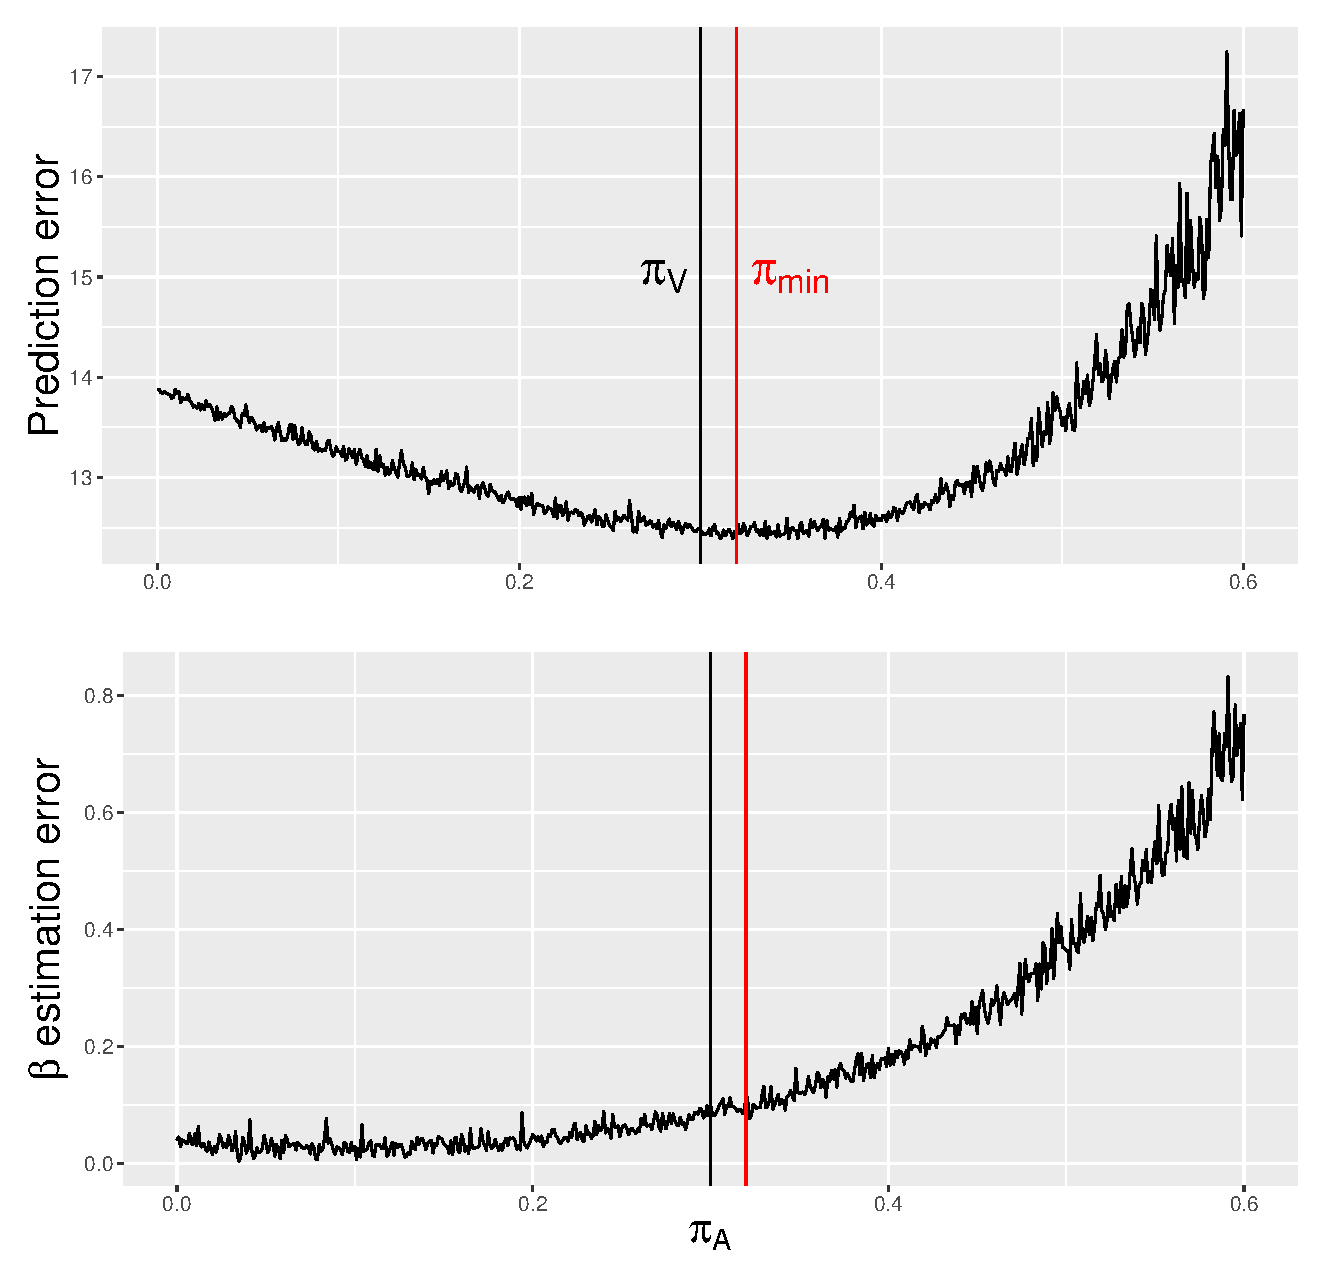
\includegraphics[scale=0.4]{Resources/miss_impact_sim}}\\
  \subbottom[Prediction error for abalone data]{%
    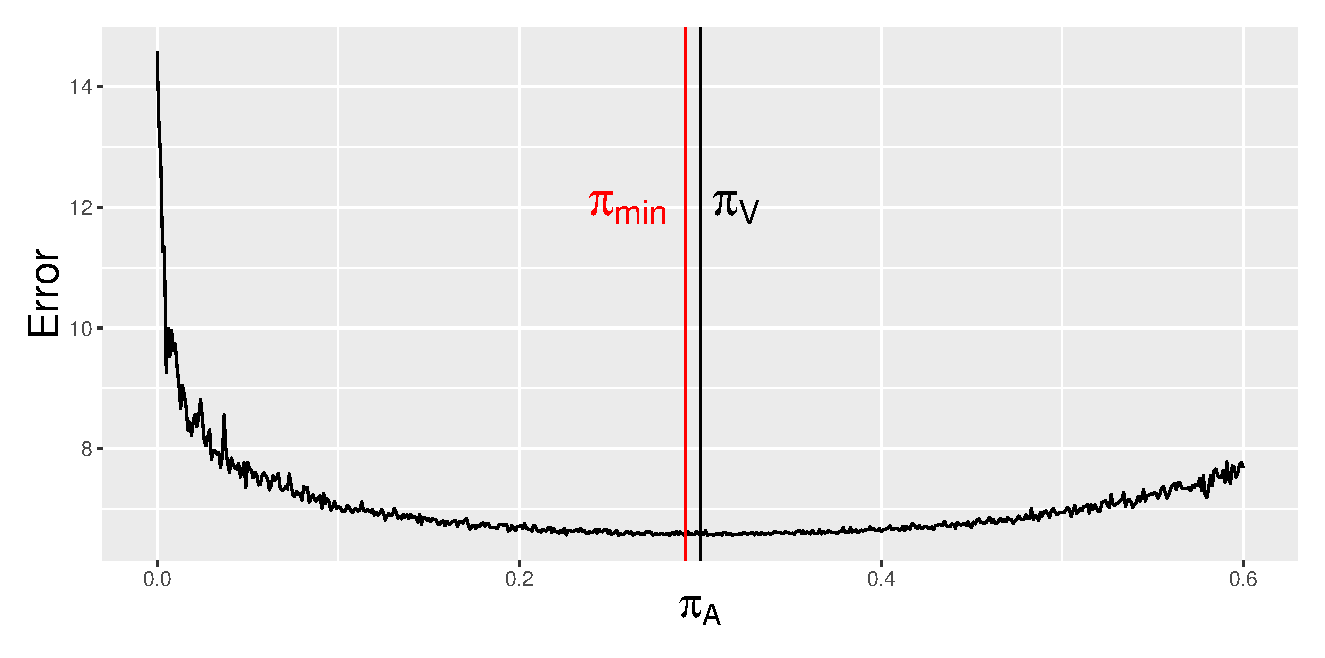
\includegraphics[scale=0.4]{Resources/miss_impact_aba}}
  \caption{Impact of missing data in the training set}
  \label{fig.miss_impact}  
\end{figure}

What we can see here is that when the training dataset is fully observed while the validation has missing data, the prediction error is \emph{higher} than in the same situation with missing data in the training set as well. More precisely, the best prediction is achieved when both datasets have roughly the same amount of missing data.

It is not clear how general this result is. In particular, we could obtain it \emph{only when using mean imputation}: with more elaborate imputation methods it did not show. 

 In any case, this warrants caution when doing cross-validation with missing data: while reducing the amount of missing data in our records is a worthy endeavour --- e.g.\ by deleting incomplete cases ---, it is possible that it will only be useful if the real-world (or validation) data also has less missing data as a result --- e.g., improving the data-collection process. Additionally, just as it is important to ensure that the distribution of the data is stable between training and application --- no temporal trend in the data ---, the same should be done about the missing-data pattern.

		\subsection{Asymmetry between the two datasets}
We want to keep investigating an observation from the previous chapter: missing data does not have the same impact on performance when it is in the training set as when it is in the validation set, and depending on the situation one or the other may be determinant of the value of the error.

To do this we simulate data in the same fashion as above, that is with a normal $X$ and a linearly derived response $y$. For various proportions $\pi$, we then perform normal imputation (cf Chapter \ref{validation}) and prediction in 4 different cases:
\begin{itemize}
\item Proportion $\pi$ of MCAR missing values in both datasets: we note the loss $L_B$
\item Proportion $\pi$ of MCAR missing values just in the validation set: we note the loss $L_V$
\item Proportion $\pi$ of MCAR missing values just in the training set: we note the loss $L_A$
\item Fully observed data: we note the loss $L_F$.
\end{itemize}

Figure \ref{fig.linreg} shows the results of this process, for simulated (cf Appendix \ref{simulation} with $p=45, rho=0.5, \sigma=1$) and real-world data (abalone, cf Appendix \ref{abalone}), adding 30\% MCAR data . We observed that the variable that caused the most change in the relationship between each type of error was $p$, the number of covariates, which is why we choose to present the results for different values of $p$. We can see that $L_B$ tends to follow the trend imposed by either $L_A$ or $L_V$, whichever is worse: when $p$ is small, $L_B$ is almost equal to $L_V$ (i.e., with few parameters to estimate the estimation of $\beta$ is good so the biggest impact is from the imputation error in $X_V$). When $p$ is larger, $L_B$ starts following the trend of $L_A$ (with many parameters to estimate, the error on $\beta$ causes very large errors to appear), although $L_B$ stays smaller than $L_A$, which is the same effect that we showed in \ref{miss_impact}.

\begin{figure}[h]
  \centering
  \subbottom[Results for simulated data (log scale)]{%
    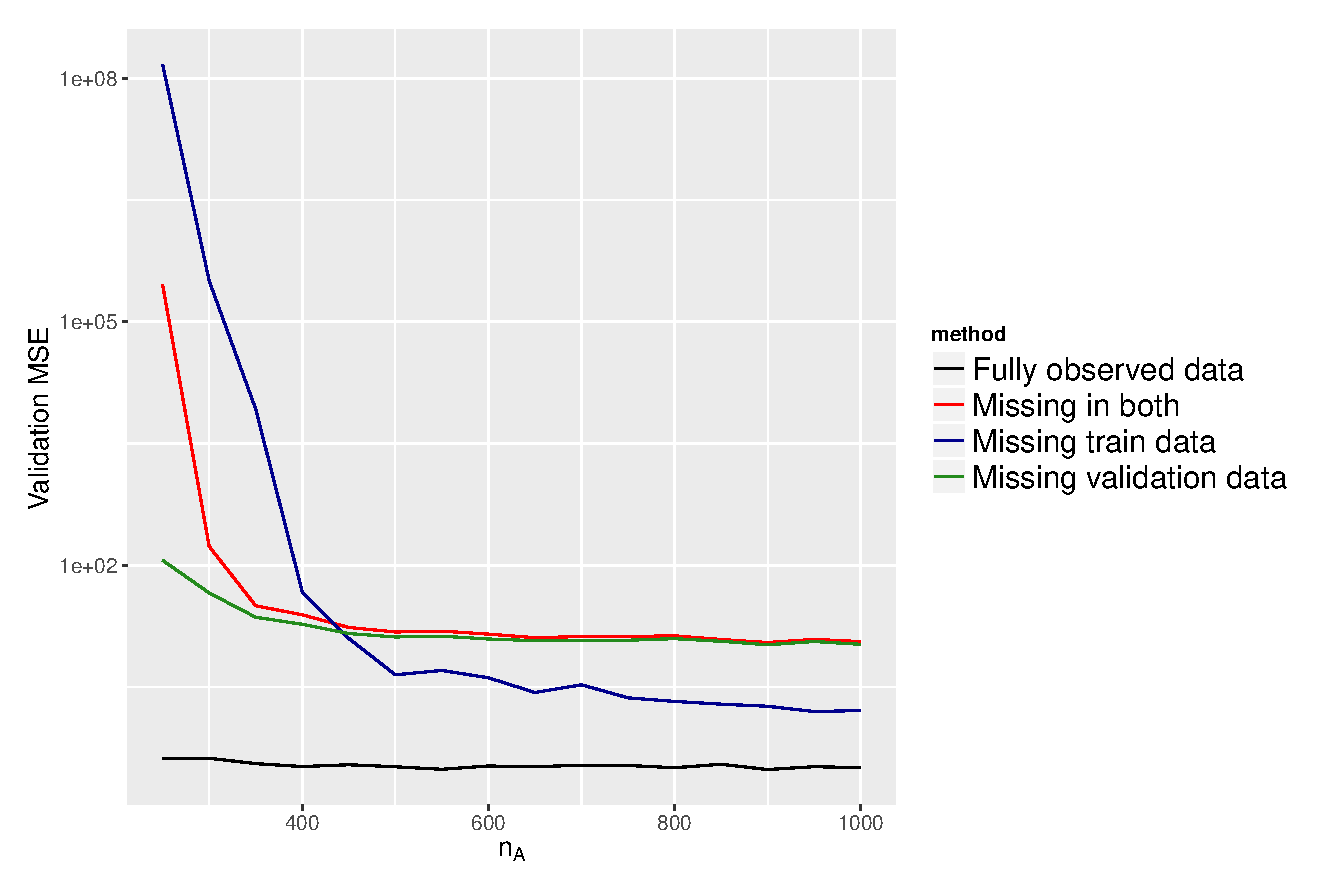
\includegraphics[scale=0.4]{Resources/linreg_sim}}\\
  \subbottom[Results for abalone data]{%
    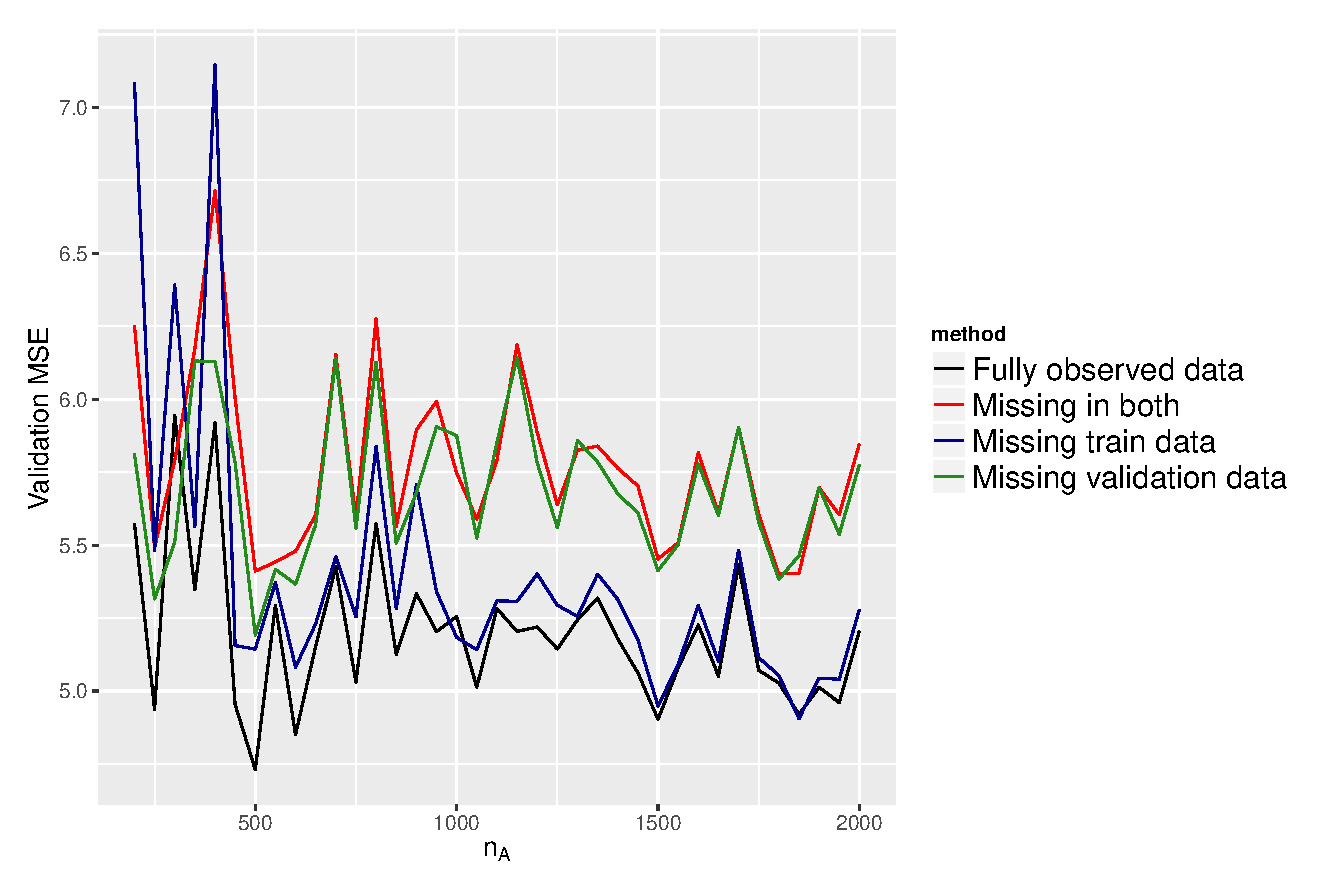
\includegraphics[scale=0.4]{Resources/linreg_abalone}}
  \caption{Impact of missing data in the train and validation set}
  \label{fig.linreg}  
\end{figure}